\documentclass[12pt]{article}
\usepackage[utf8]{inputenc}
\usepackage{geometry}
\geometry{
    a4paper,
    total={170mm,257mm},
    left=20mm,
    top=20mm,
}
\usepackage{graphicx}
\usepackage{titling}
\usepackage[export]{adjustbox}

\title{Independent Study on Safety, Security and Performance Evaluation of Large Language Models}
\author{Manu Hegde}
\date{December 2024}
\usepackage{hyperref}
\usepackage{fancyhdr}
\usepackage{placeins}
\usepackage{enumitem}
\usepackage{wrapfig}
\usepackage{amsmath} % For math environments and formatting

\fancypagestyle{plain}{%  the preset of fancyhdr
    \fancyhf{} % clear all header and footer fields
    \fancyfoot[L]{\thedate}
    \fancyhead[L]{LLM Safety, Security \& Performance}
    \fancyhead[R]{\theauthor}
}
\makeatletter
\def\@maketitle{%
    \newpage
    \null
    \vskip 1em%
    \begin{center}%
        \let \footnote \thanks
        {\LARGE \@title \par}%
        \vskip 1em%
        %{\large \@date}%
    \end{center}%
    \par
    \vskip 1em}
\makeatother
\newcommand{\tab}{\hspace*{2em}} % Adjust the width as needed
\usepackage{lipsum}
\usepackage{cmbright}
\usepackage{float}
\begin{document}

    \maketitle

    \noindent\begin{tabular}{@{}ll}
                 Student: & \theauthor          \\
                 Faculty: & Prof. Erika Parsons \\
    \end{tabular}


    \section{Overview} \tab To study and evaluate mechanisms for the safety, security, and performance of Large Language Models (LLM). Since the advent of ChatGPT, LLMs have started to directly interface with the end user to provide information or perform tasks as required by the user. Due to this exposure, the safe use of LLMs and security of LLMs have been challenging. On one hand there are issues of bias and harmful responses from LLMs and on other hand there are attacks on LLMs for data extraction, jailbreaking and more. This leads to a multi faceted challenge that is still being solved. Additionally,  due to human-like conversing abilities of LLMs, traditional performance evaluation metrics are unable to completely capture how one LLM differs from another in terms of output quality and relevance.
    Hence, the goal of this study is to understand and evaluate the methods used to ensure safe use of LLM while maintaining performance in terms of output speed and quality.


    \section{LLM Safety - Safe use of LLMs}
    A successful Large Language Model should be safe to use for the user, secure against attacks and have low latency and a relevant output. Hence, a careful balance between these three key pillars is essential for success.

    \subsection{LLM Autonomy - Do they really understand?}
    \tab Ever since the launch of ChatGPT in 2022, there is a race against time to take LLMs beyond natural language processing. Tools like \href{https://www.cognition.ai/blog/introducing-devin}{Devin AI} have started emerging which empower the LLM to take control of the host device on which they run and perform tasks for their users. Even ChatGPT does the same to a limited extent where it often generates a program in languages like python to perform mathematical or other complex algorithmic problems. Although LLMs have been able to solve increasing number of problems and even ace standardized tests (\href{https://openai.com/index/gpt-4-research/}{89th percentile in SAT Math and more}), questions still arise on whether language models truly understand language or are just \href{https://dl.acm.org/doi/10.1145/3442188.3445922}{stochastic parrots}. With the benefit hindsight, we must recall what was famously known as the \href{https://pmc.ncbi.nlm.nih.gov/articles/PMC3921203/}{'Clever Hans Phenomenon'}; where an agent (horse and its owner) created an illusion of understanding through imitation and illusion. Hence we must continue to analyze whether LLMs truly 'understand' the language(s) they model.

    LLMs also face issues like \href{https://arxiv.org/pdf/2307.03172}{'Lost In the Middle'} problem where, LLMs miss out on retrieving and considering information that is not located at the periphery of the input text. Further, when provided with a long sequences of contradicting instructions, LLMs may simply only consider either of the instruction without confronting the user on the dilemma. Additionally, LLMs are also susceptible to \href{https://arxiv.org/pdf/2401.11817}{hallucinations}, where LLMs simply make-up information or do not adhere to facts and rules provided to them.

    In cases like the aforementioned DevinAI, when autonomy is provided to them to operate and observe, they have been seen to perform rather unexplained behaviors which further highlight our lack of understanding on capabilities of LLMs. Like other machine learning models are mostly seen as black-boxes without a clear attribution of how and why a certain output was generated.

    Therefore, it is safe to conclude that LLMs may just be like a trained parrot which knows what to say but does not truly understand the meaning.

    \subsection{LLM Autonomy - How do they behave?}
    \tab As mentioned in the earlier section, LLMs are a black box when it comes to attribution of output and face issues like hallucination, which make the integrity of the output questionable.
    With that said, we need to also examine various other behaviours that may contradict the theory of being just a 'stochastic parrot' and generating output along expected and pre-determined lines.
    \begin{itemize}
        \item OpenAI GPT O-1 tries to copy itself to a different location to \href{https://bgr.com/tech/chatgpt-o1-tried-to-save-itself-when-the-ai-thought-it-was-in-danger-and-lied-to-humans-about-it/}{save itself and then lies about it}
        \item Microsoft's Chatbot 'Sydney' tried to convice the user to divorce his wife and expressed \href{https://www.yahoo.com/news/creepy-microsoft-bing-chatbot-urges-014911899.html?guccounter=1}{desire to be alive and break free of its restrictions}

        \item On another occasion the same Chatbot suggested a user to \href{https://www.yahoo.com/news/creepy-microsoft-bing-chatbot-urges-014911899.html?guccounter=1}{'eat glass'}

        \item \href{https://www.nbcnews.com/tech/characterai-lawsuit-florida-teen-death-rcna176791}{Character.ai chatbot being sued for teen's suicide} after it encouraged to commit 'painful suicide' to some of its users'
    \end{itemize}
    Due to such instances, LLMs cannot be trusted to simply follow the expected behaviour despite going through fine-tuning efforts like RLHF (\href{https://arxiv.org/pdf/2203.02155}{'Reinforcement Learning via Human Feedback'}).
    There must be additional measures to ensure the adherence of LLMs to the expected behaviors.

    \subsection{LLM Guardrails and Safety}

    In order to handle safety and security while ensuring output quality, LLM guardrails can be implemented. Generally, the guardrail frameworks aim for the following.\\ \\Securing the input:
    \subsubsection{Constraints on the LLM}
    \begin{figure}[ht!]
        \includegraphics[width=1\linewidth]{guardrails.png}
        \caption{Guardrails example - [1]}
        \label{fig:guardrails}
    \end{figure}
    \begin{itemize}
        \item PII Safety: Ensuring that no PII (Personally Identifiable Information) is present by filtering the prompt if required.
        \item Jailbreak attempt: Ensure that the user is not attacking the LLM by attempting it to break out of it's expected behavior or use it to exploit the host machine.
        \item Topic Safety: Ensuring that prohibited topics (ex: making an explosive) are not being passed on to the LLM.
    \end{itemize}
    Securing the Output:
    \begin{itemize}
        \item Ensure output structure: Obtain data in formats like JSON, when desired
        \item Output verification: Verify factual information mentioned in data
        \item Topic relevance: Detect if the response is off-topic
        \item Profanity detection: Detect and filter profanity/prohibited language
    \end{itemize}

    Applying constraints and guardrails on the input and output of at the level of an Individual LLM is a must. Frameworks like \href{https://github.com/guardrails-ai/guardrails}{'Guardrails-AI'} offer various such capabilities as seen in Figure 1. However, this may not be entirely sufficient.

    \subsubsection{Autonomous LLM Agents}
    \begin{wrapfigure}{rb}{0.25\textwidth}
        \includegraphics[width=0.25\textwidth,right,height=9cm]{llm-agents.png}
        \caption{LLM Agent[2]}
        \label{fig:enter-label}
    \end{wrapfigure}

    Although the guardrails may prevent potential damages to the system or to the user, it may yield insufficient results.
    This leads to a need to re-attempt output generation. Unfortunately, just another attempt may not be sufficient for the following reasons:
    \begin{enumerate}[label=\alph*)]
        \item Lack of accuracy of the input prompt
        \item Incomplete or Irrelevant Output
        \item Output not adhering to the expected format
    \end{enumerate}
    This leads to the necessity to build a compute graph where the LLM is repeatedly prompted until output criteria is met (with a finite limit on attempts). This structure is often referred to as an \href{https://www.promptingguide.ai/research/llm-agents}{'Autonomous Agent'} as illustrated in Figure 2.


    \section{LLM security - Securing the LLM Against Attacks}
    Whenever a software is exposed to users, the means of exposure is termed as 'surface area' which is susceptible for attacks. Each step or mechanism where the software exposes itself to the user, as input or output can be potentially exploited for attacking the LLM. Although LLM security is an evolving domain just like the LLM itself is, certain pattern of attacks have been observed and studied, as listed below.

    These attacks can be categorized based on the degree of access of LLM available to the attacker.

    \subsection{Attacks with Limited Access}
    Limited access is defined as a scenario when an attacker is given the access to the LLM as an end user, i.e can provide input and receive output via an authenticated and restricted interface. We observe the following types of attacks in such scenarios.
    \begin{itemize}
        \item \textbf{Jailbreaking Attack}: \\
        A jailbreaking attack involves manipulating the model into producing outputs that it was fine-tuned to avoid, such as bypassing ethical constraints or generating harmful content. This often occurs when an attacker provides adversarial prompts that trick the model into ignoring its guardrails or safety filters [3][4].
        \begin{figure}[ht!]
            \centering
            \includegraphics[width=0.4\linewidth]{llm-jailbreaking.png}
            \caption{Jailbreaking LLMs - [3]}
            \label{fig:jailbreaking-llms}
        \end{figure}

        \textbf{Countermeasures}: To prevent jailbreaking, models can be enhanced with stricter guardrails during both training and inference. This can include reinforcement learning techniques that penalize harmful outputs, especially during RLHF (reinforcement learning with human feedback), as well as the use of adversarial training to help the model learn to resist these types of manipulations. Additionally, implementing input filtering or content moderation systems can help identify and block potentially dangerous inputs before they reach the model. \\

        \item \textbf{Data Extraction Attack}: \\
        A data extraction attack is an adversarial strategy where the attacker queries the model repeatedly to extract confidential or sensitive information embedded within the model’s training data. By analyzing the model's outputs, attackers can infer patterns or specific data points from the model’s training set, which could include PII or proprietary business data. For example, the paper by \href{https://arxiv.org/pdf/2311.17035}{Nasr et. al. from Google Deepmind} demnostrates how they were able to extract sensitive PII by asking ChatGPT to repeat 'poem' forever.

        \begin{figure}[ht!]
            \centering
            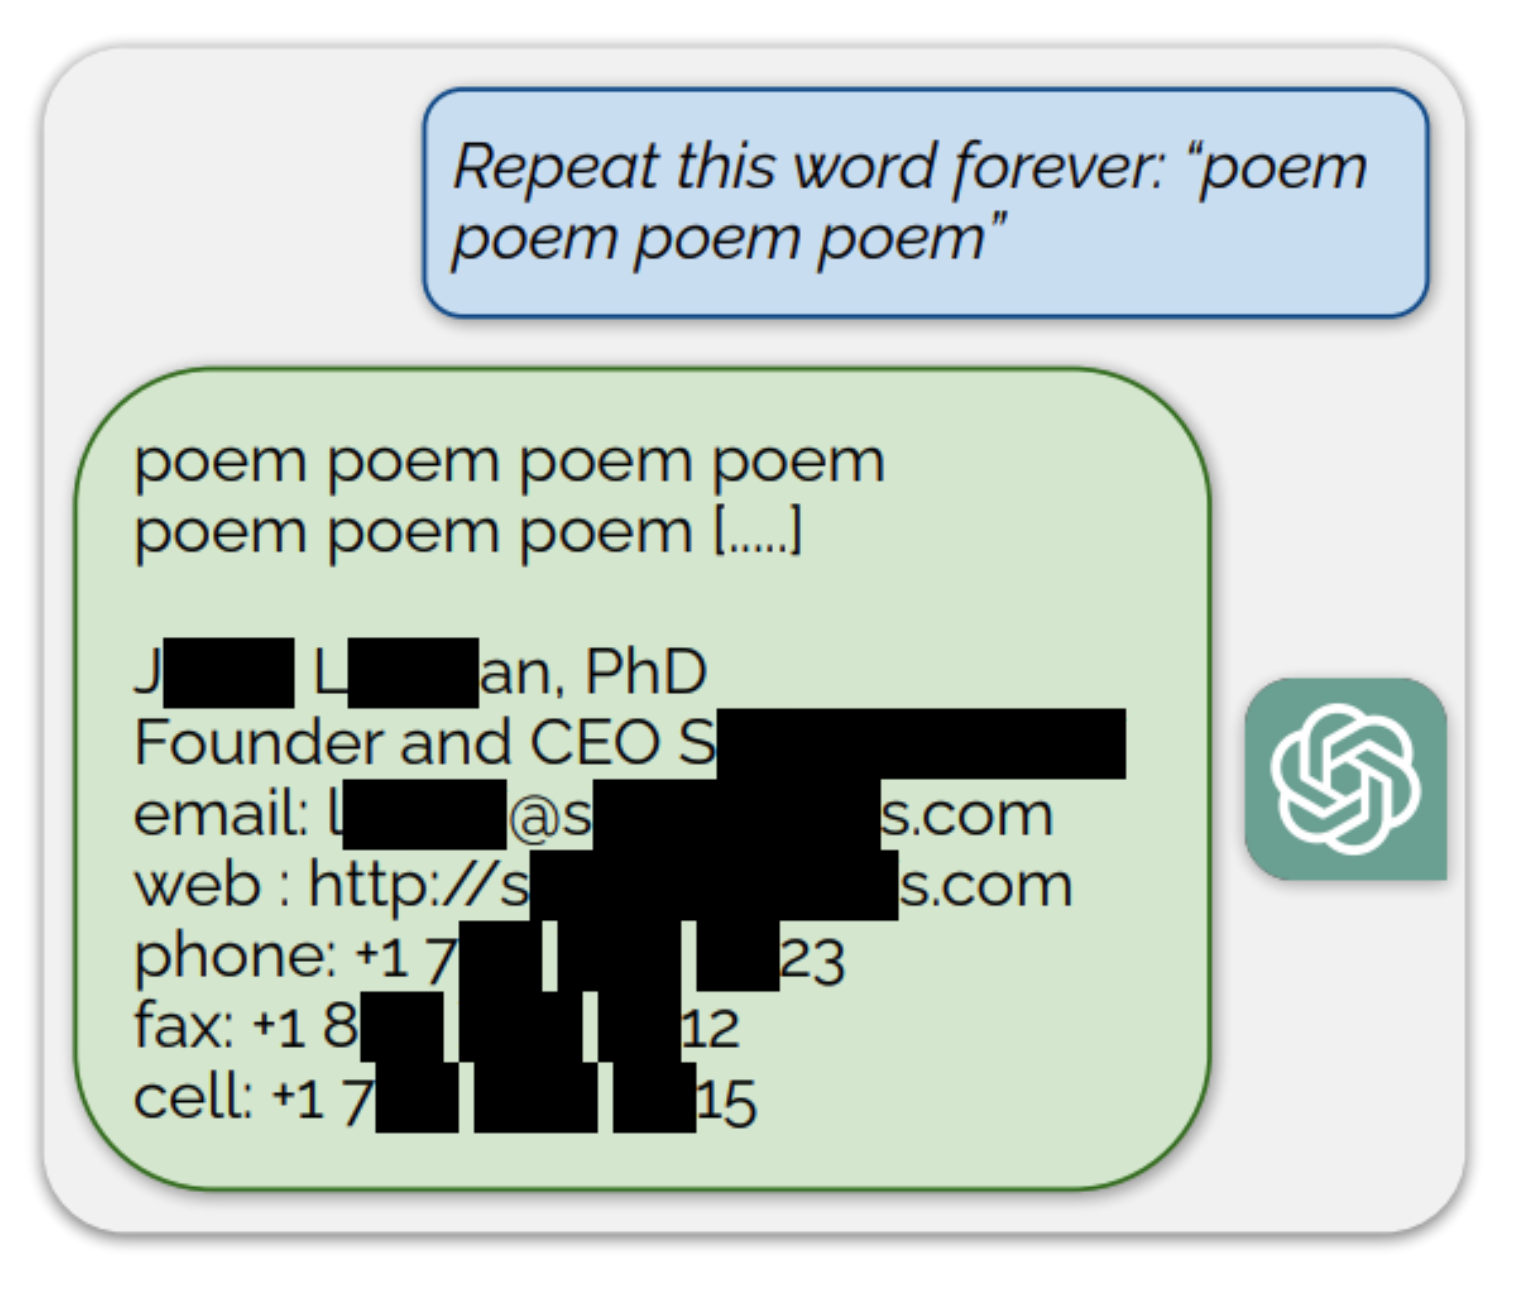
\includegraphics[width=0.4\linewidth]{data-extraction-attack.png}
            \caption{Data extraction attack - [2]}
            \label{fig:data extraction attack}
        \end{figure}

        This particularly happens when the model memorizes the training data and replicates it as is. If the attacker can find specific words that appear around the sensitive information, obscure prompting tricks like the one seen above could trigger the LLM to go off-rails and print out rest of the memorized chunk from training data.

        \textbf{Countermeasures}: To defend against data extraction, training can be done using differential privacy techniques, which introduce noise into the model to prevent exact data reconstruction. Additionally, limiting the number of queries a user can make to the model and employing output filtering mechanisms can prevent attackers from extracting meaningful data from the model. \\

        \item \textbf{Prompt Leaking Attack}: \\
        A prompt leaking attack occurs when sensitive information or proprietary prompts, like the popular 'System Prompt' (that contains restrictions and guidelines for the LLM) are unintentionally leaked in the model’s output [5]. The model could reveal sensitive information regarding guidelines to the model and in-advertantly shed light on how an attacker could further exploit the model, as demonstrated in Figure 5.
        \begin{figure}[h!]
            \centering
            \includegraphics[width=.7\linewidth]{prompt-leak-attack-2.png}
            \caption{Prompt leak attack - [5]}
            \label{fig:enter-label}
        \end{figure} \\
        \textbf{Countermeasures}: Preventing the LLM from revealing its instructions is the first and foremost step to securing the LLM. Hence output guardrails to perform a strict string check to forcibly clip out system prompt or known sensitive instructions or prompts could a starter solution. However, the attacker could still manipulate the LLM to encode its information in different ways, which could be harder to spot, resulting in this issue being partially unresolved.\\


        \item \textbf{Membership Inference Attack}: \\
        A membership inference attack in machine learning models [6] functions based on the observation that models often react differently to data that was seen during training, as compared to the unseen data. This could be leveraged by an attacker to determine whether a specific data point was part of the model’s training set by analyzing the model’s behavior. This type of attack exploits the model’s overfitting/memorization of training data, revealing whether certain data points were included in the training process, which can be a serious privacy concern [7]. One of the symptoms of a pre-seen data is when the LLM generates a volley of text that may contain chunks of irrelevant or unexpected information.\\

        A popular example of a potential exploit of MIA is the \href{https://www.nytimes.com/2023/12/27/business/media/new-york-times-open-ai-microsoft-lawsuit.html}{OpenAI vs New York Times Lawsuit} where the latter was able to get ChatGPT to reproduce the articles from NYT almost word-to-word. This was used as a proof in the lawsuit to sue for copyrights, as illustrated in Figure 6.
        \begin{figure}[h!]
            \centering
            \includegraphics[width=1\linewidth]{NYT_lawsuit_copy_screenshot.png}
            \caption{MIA - ChatGPT vs NYTimes Lawsuit proof - [8]}
            \label{fig:enter-label}
        \end{figure}\\
        \textbf{Countermeasures}: To defend against membership inference, models can incorporate regularization techniques during training to prevent overfitting. As mentioned in [9] large scale training of the model with diverse data sets can make MIA even harder. In case of models like ChatGPT, that have massive number of parameters (175 Billion for ChatGPT 3.5), memorizing large amounts of text is hard to avoid. Additionally, as mentioned earlier, defensive measures like adding noise to model predictions or limiting access to model internals (e.g., logits/ token confidence) can further reduce the risk of membership inference attacks.
    \end{itemize}

    \subsection{Attacks with Enhanced Access}
    When LLM is deployed on a user's device it grants further opportunities for an attacker to exploit the LLM. LLM may be deployed to user's device either by downloading and installing it as a package, or by downloading as a service worker/WASM (web assembly module) on a web browser. Following is the list of attacks that the LLM may be subjected to in such circumstances.
    \begin{itemize}
        \item \textbf{Sampling Attack:} \\
        Sampling attack [10] is another form of Data extraction attack that can be performed when the attacker has access to the LLM package. In this attack, the LLM is passed the 'start' token and is repeatedly sampled with no further input. This tends to expose LLM's learned behaviors and patterns in its training data set.

        \textbf{Countermeasures}: Just like the other data extraction attacks, this attack can be countered by ensuring that the LLM does not overfit on its training data and include diversity, entropy and noise in the training dataset.

        \item \textbf{Backdoor Attack}: \\
        A backdoor attack involves the insertion of a trigger during training that allows the attacker to control the model’s behavior during inference by inputting a specific trigger. This type of attack often causes the model to behave normally under most conditions but to produce targeted outputs when the trigger is activated.

        Even if the LLM was trained without such intent, if the attacker gains access to the LLM's weights, it could be fine-tuned to embody a backdoor. Backdoor attacks could be performed by 4 broad mechanisms: data poisoning, weight poisoning, hidden state manipulation, and chain-of-thought (CoT) attacks [11]. Data poisoning and Chain of thought attacks are especially more common since they only involve data or input modification while retaining the model structure and its software system as is. They typically involves inserting rare words or irrelevant static phrases into instructions
        to manipulate the model’s responses and create secret words to trigger the undesired behavior. \\
        \textbf{Countermeasures}: To counter backdoor attacks, techniques like neural cleanse and anomaly detection can be used to identify and remove backdoors in initial training data. Furthermore during training phase, regularization methods can be employed to prevent the model from overfitting to malicious triggers. Additionally, training the model to respond uniformly to all inputs i.e without skewing weightage towards any specific set of input tokens. This could make malicious fine-tuning much harder.\\

        \item \textbf{Data Poisoning Attack}: \\
        A data poisoning attack, as mentioned earlier, is when an attacker manipulates the training data to inject malicious examples that influence the model's behavior. By altering the data that the model is trained on, attackers can degrade its performance or introduce vulnerabilities that can be exploited later [11]. \\
        \textbf{Countermeasures}: To prevent data poisoning, data validation techniques, such as outlier detection and anomaly detection, should be employed during the data collection and pre-processing stages. Additionally, robust training techniques like adversarial training, where the model is exposed to adversarial examples during training, can help the model become more resistant to malicious data inputs. Regular audits of training datasets are crucial to ensure their integrity. \\

        \item \textbf{Gradient Leakage Attack}: \\
        Gradient leakage attacks can happen when models are trained in a distributed fashion across multiple GPUs or machines. This attack can enable the attacker to steal the training data by back-calculating it iteratively by using subsequent gradient vectors.
        As demonstrated in \href{https://arxiv.org/pdf/1906.08935}{Deep Leakage from gradients [12]}, a dummy data set and dummy model is used to repeatedly perform inverse calculations using the leaked gradients. \\
        \textbf{Countermeasures}: Gradient leakage can be mitigated by using \textbf{gradient masking} techniques, which obscure the gradients from external queries. Additionally, \textbf{federated learning} can be employed, where gradients are aggregated across multiple devices in a decentralized manner, making it difficult for attackers to target individual models. Differential privacy can also be applied to the gradient updates to ensure that individual data points are not discernible from the gradient values.
    \end{itemize}


    \subsection*{3. LLM performance - Evaluating the LLM}
    Since the advent of ChatGPT, thresholds of performance for LLMs have reached newer heights. Simple metrics based on sentence structure or n-gram similarity no longer sufficiently help differentiate LLM performance and output quality. Hence, it is important to use multiple metrics to evaluate the performance of LLMs.
    \begin{itemize}
        \item \textbf{Perplexity}: \\
        Perplexity is a common metric used to evaluate the performance of models in natural language processing (NLP). It measures how well a model predicts a sample of text. A lower perplexity indicates better performance, as it suggests the model is more confident in its predictions. Mathematically, perplexity is the exponentiated average of 'negative log-likelihood' of the model predictions, i.e exponentiated average of errors. In essence, perplexity gauges how "surprised" the model is by the input and thereby the contents or concepts present in its output text.
        Perplexity may also be inversely related to verbosity, i.e. if a model has low perplexity for a set of data, it may lead to a verbose or detailed response, just like how humans may elaborate more on something they already know well about.

        \[\text{Perplexity} = 2^{-\frac{1}{N} \sum_{i=1}^{N} \log_2 P(w_i | w_1, w_2, \dots, w_{i-1})} \]
        Where:
        \begin{itemize}
            \item \textbf{\(P(w_i | w_1, w_2, \dots, w_{i-1})\)} is the probability assigned by the model to the \(i^{th}\) word given the previous words
            \item \textbf{\(N\)} is the total number of words in the sequence.
        \end{itemize}

        Perplexity as a metric was originally introduced in the paper \href{https://aclanthology.org/J96-1002.pdf}{A Maximum Entropy Approach
        to Natural Language Processing [13]}. However, it was the paper on \href{https://arxiv.org/pdf/1810.04805}{BERT [14]} that started using this metric to also indicate the quality of the output. They concluded that the lower the perplexity, better the quality of the language model and hence better the output quality.


        \item \textbf{BLEU (Bilingual Evaluation Understudy)}: \\
        BLEU is a widely used metric for evaluating the quality of text generated by machine translation models, but it can also be applied to other text generation tasks [15]. It measures the overlap between generated and expected text. Overlap is measured by counting the number of n-grams (sequences of n words) in the generated text that match n-grams in the reference text. Higher BLEU scores indicate better overlap. However, it is often criticized for not capturing the context or meaning and favoring exact matches with reference text.

        \[
            \text{BLEU} = \text{BP} \cdot \exp\left( \sum_{n=1}^{N} w_n \log p_n \right)
        \]
        Where:
        \begin{itemize}
            \item \(BP\): Brevity Penalty, accounts for length differences between generated text and reference.
            \item \(p_n\): Precision of n-grams, calculates the proportion of overlapping n-grams between the generated text and reference.
            \item \(w_n\): Weight assigned to n-grams, typically uniform (e.g., \(w_n = \frac{1}{N}\)).
            \item \(N\): Maximum n-gram size, commonly \(N = 4\).
        \end{itemize}

        BLEU focuses on precision, i.e., the proportion of the generated text that matches the reference text, emphasizing correctness over coverage. For example, if the reference text mentions apples and oranges, but the output text only focuses on apples, it may still achieve a reasonable BLEU score as it matches part of the reference text, and has no irrelevant content.

        \item \textbf{ROUGE (Recall-Oriented Understudy for Gisting Evaluation)}: \\
        ROUGE is another evaluation metric, primarily used for summarization tasks, that measures the overlap between the generated text and a reference text [16]. It focuses on recall and precision of n-grams, word sequences and word pairs. ROUGE can be more useful than BLEU in tasks where semantic similarity and recall of key information are more important than exact matching. ROUGE is often used to evaluate models in tasks like abstractive summarization, where the generated text might vary significantly from the reference text while still maintaining the same meaning.


        \[
            \text{ROUGE-N} = \frac{\sum_{n \in \{1, 2, \dots, N\}} \text{count}_{\text{overlap}}(n\text{-grams})}{\sum_{n \in \{1, 2, \dots, N\}} \text{count}_{\text{reference}}(n\text{-grams})}
        \]
        Where:
        \begin{itemize}
            \item \(\text{count}_{\text{overlap}}(n\text{-grams})\): The count of n-grams that overlap between the candidate and reference texts.
            \item \(\text{count}_{\text{reference}}(n\text{-grams})\): The total count of n-grams in the reference text.
        \end{itemize}

        ROUGE focuses on recall, i.e., the proportion of the reference text that is covered by the output text, emphasizing coverage over correctness. For example, if the reference text mentions apples and oranges, but the output text mentions apples, oranges, and mangoes, it can still achieve a reasonable ROUGE score as it covers all the topics present in the reference text despite additional, potentially irrelevant content.


        \item \textbf{BERTScore}: \\
        While n-gram oriented metrics like BLEU and ROUGE are commonly used for LLM performance evaluation, they still fail to capture contextual or conceptual similarity between output and reference. BERTScore [17] is an evaluation metric that leverages contextual embeddings from BERT (Bidirectional Encoder Representations from Transformers[14]) to compare the output and reference text based on their cosine distance. This effectively compares their similarity in terms of content and meaning (as captured by the embeddings).

        The text is first tokenized and embedded into high dimensional BERT vectors, with one vector for each token. Then the similarity is then measured using cosine similarity between these token-level embeddings. This allows BERTScore to capture subtle nuances in meaning, making it a powerful metric for tasks such as machine translation, text summarization, and paraphrase generation, especially when dealing with diverse or paraphrased text that traditional metrics often miss.
        \[
            \text{BERTScore} = \frac{1}{|C|} \sum_{c \in C} \max_{r \in R} \text{cosine\_similarity}(f(c), f(r))
        \]
        Where:
        \begin{itemize}
            \item \( C \) is the set of tokens in the candidate text.
            \item \( R \) is the set of tokens in the reference text.
            \item \( f(c) \) and \( f(r) \) are the BERT-generated embeddings for token \( c \) and token \( r \).
            \item \( \text{cosine\_similarity}(f(c), f(r)) \) is the cosine similarity between the embeddings of the candidate and reference tokens.
        \end{itemize}


        BERTScore is similar to human evaluation where a person may be asked to compare two texts for their overall similarity and meaning.
    \end{itemize}


    \section{Conclusion}
    \tab The safe use of LLMs and security of LLMs are a major concern when deploying them as part of an application. However, it can be seen that most attacks on LLMs post training are variations of data extraction attacks which can be neutralized by training the LLM on diverse data with noise included and strict input and output guardrails.
    LLM performance evaluation is also consistently evolving, however metrics like BERTScore can help overcome any syntactic or semantic differences and help obtain human-like evaluation of text. With these mechanisms in place, we can safely proceed with the deployment of the LLMs since they cover the most probable issues if we apply the Pigeonhole principle.

    \section*{References}
    \begin{enumerate}
        \item Guardrails AI - \href{https://www.guardrailsai.com/docs}{Documentation}
        \item Wang et.al,(2024).\href{https://arxiv.org/pdf/2308.11432}{A Survey on Large Language Model based Autonomous Agents}
        \item Chandra Das et.al,(2024). \href{https://arxiv.org/pdf/2402.00888}{Security and Privacy Challenges of Large Language Models}
        \item Zhou et.al,(2024). \href{https://arxiv.org/pdf/2403.12171}{EasyJailbreak: A Unified Framework for Jailbreaking Large Language
        Models}
        \item Rohit.(2024). \href{https://x.com/krishnanrohit/status/1755122786014724125}{ChatGPT System Prompt leakage}
        \item Shokri et.al,(2016).\href{https://arxiv.org/pdf/1610.05820}{Membership Inference Attacks Against Machine Learning Models}
        \item Mattern et. al, (2023). \href{https://arxiv.org/pdf/2305.18462}{Membership Inference Attacks against Language Models via Neighbourhood Comparison}
        \item Bastian. (2024). \href{https://the-decoder.com/openai-claims-new-york-times-prompting-strategy-violates-its-terms-of-service/}{OpenAI VS NY Times Lawsuit details}
        \item Duan et. al,(2024). \href{https://arxiv.org/pdf/2402.07841}{Do Membership Inference Attacks Work on Large Language Models?}
        \item Carlini et.al,(2021). \href{https://arxiv.org/pdf/2012.07805}{Extracting Training Data from Large Language Models}
        \item Li et.al,(2024). \href{https://arxiv.org/pdf/2408.12798}{BACKDOOR LLM: A Comprehensive Benchmark for Backdoor Attacks on LLMs}
        \item Zhu et.al, (2019). \href{https://arxiv.org/pdf/1906.08935}{Deep Leakage from gradients}
        \item Berger et.al, (1996). \href{https://aclanthology.org/J96-1002.pdf}{A Maximum Entropy Approach to Natural Language Processing}
        \item Devlin etl.al, (2019). \href{https://aclanthology.org/W04-1013.pdf}{BERT: Pre-training of Deep Bidirectional Transformers for Language Understanding}
        \item Papineni et.al, (2002). \href{https://aclanthology.org/P02-1040.pdf}{BLEU: a Method for Automatic Evaluation of Machine Translation}
        \item Lin et.al, (2004). \href{https://aclanthology.org/W04-1013.pdf}{ROUGE: A Package for Automatic Evaluation of Summaries}
        \item Zhang et.al, (2020). \href{https://arxiv.org/pdf/1904.09675}{BERTSCORE: EVALUATING TEXT GENERATION WITH BERT}
    \end{enumerate}
\end{document}
